% ====================================================================
%  Chapter 5: Multi-User Behavior Learning System
% ====================================================================
\newpage
\section{Multi-User Behavior Learning System}
\label{sec:behavior-learning}

\subsection{Introduction and Motivation}

Smart home systems traditionally rely on rule-based automation: if temperature exceeds threshold, trigger alert; if time matches schedule, execute action. While deterministic and predictable, such approaches cannot adapt to individual user preferences or learn from behavioral patterns.

This chapter presents a machine learning system that observes user interactions with smart home devices and learns personalized behavioral models. The system addresses two key limitations of rule-based approaches:

\begin{enumerate}
    \item \textbf{Implicit preference learning:} Users rarely configure hundreds of preference parameters. Instead, the system infers preferences from natural usage patterns (e.g., Dad consistently turns on living room light at 70\% brightness around 6:30 AM).
    
    \item \textbf{Context-dependent behavior:} The same action may have different meanings in different contexts. A user's lighting preference at 6:30 AM (bright for morning routine) differs from 10:00 PM (dim for relaxation). Rule-based systems cannot easily capture such contextual nuances.
\end{enumerate}

The chapter is organized into two parts: \textbf{Part A} focuses on the machine learning model (architecture, training, evaluation), while \textbf{Part B} addresses system engineering challenges (multi-user handling, integration with existing HERA agents).

\subsection{Problem Formulation}
\label{sec:problem-formulation}

Given a household with $N$ users $U = \{u_1, u_2, \ldots, u_N\}$ and $M$ controllable devices $D = \{d_1, d_2, \ldots, d_M\}$, the system observes a sequence of user actions:

\begin{equation}
    A = \{(u_i, d_j, s_j, t, c) \mid u_i \in U, d_j \in D, t \in \mathbb{R}^+, c \in \mathcal{C}\}
\end{equation}

where:
\begin{itemize}
    \item $u_i$ is the user performing the action
    \item $d_j$ is the target device
    \item $s_j$ is the desired device state (e.g., brightness level, on/off)
    \item $t$ is the timestamp
    \item $c$ is the environmental context (temperature, humidity, current device states)
\end{itemize}

The learning objective is to train per-user models $f_{u_i}$ that predict:

\begin{enumerate}
    \item \textbf{Next device prediction} (classification): Which device is user $u_i$ most likely to control next, given context $c$ and time $t$?
    \begin{equation}
        P(d_j \mid u_i, c, t) = f_{u_i}^{\text{device}}(c, t)
    \end{equation}
    
    \item \textbf{Preferred device state} (regression/classification): What is user $u_i$'s preferred state for device $d_j$ in context $c$?
    \begin{equation}
        \hat{s}_j = f_{u_i}^{\text{state}}(d_j, c, t)
    \end{equation}
\end{enumerate}

These predictions enable both \emph{reactive personalization} (applying learned preferences when user issues ambiguous commands like ``turn on light'' without specifying brightness) and \emph{proactive suggestions} (``Good morning! Turn on living room light? You usually do at this time.'').

%%%%%%%%%%%%%%%%%%%%%%%%%%%%%%%%%%%%%%%%%%%%%%%%%%%%%%%%%%%%%%%%%%%%%%%
% PART A: MACHINE LEARNING MODEL
%%%%%%%%%%%%%%%%%%%%%%%%%%%%%%%%%%%%%%%%%%%%%%%%%%%%%%%%%%%%%%%%%%%%%%%

\subsection*{\Large PART A: MACHINE LEARNING MODEL}
\addcontentsline{toc}{subsection}{Part A: Machine Learning Model}

\subsection{Model Architecture Selection}
\label{sec:model-selection}

\subsubsection{Design constraints}

The model must satisfy several practical constraints for deployment in a family smart home backend:

\begin{itemize}
    \item \textbf{Small dataset regime:} Each user generates 10--50 device control actions per day. After 30 days of collection, training datasets contain only 300--1500 samples per user.
    
    \item \textbf{Low-latency inference:} Predictions must complete within 50ms to avoid adding perceptible delay to the conversational interface.
    
    \item \textbf{Interpretability:} For user trust and debugging, the model should provide feature importance rankings to explain why certain predictions were made.
    
    \item \textbf{Continuous learning:} Models must be retrained nightly on new data without manual intervention.
\end{itemize}

\subsubsection{Model comparison}

Table~\ref{tab:model-selection-comparison} compares candidate model architectures evaluated for this task.

\begin{table}[H]
    \centering
    \caption{Model architecture comparison for behavior prediction task.}
    \label{tab:model-selection-comparison}
    \renewcommand{\arraystretch}{1.3}
    \small
    \begin{tabularx}{\textwidth}{@{} >{\raggedright\arraybackslash}p{2.2cm} X X X @{}}
        \toprule
        \textbf{Model} & \textbf{Advantages} & \textbf{Limitations} & \textbf{Suitability} \\
        \midrule
        
        Logistic Regression &
        Fast, interpretable, proven baseline for behavior prediction \cite{richardson_predicting_2007}. &
        Assumes linear decision boundaries. Cannot model interactions between temporal and environmental features. &
        Baseline only. Insufficient for context-dependent patterns. \\
        
        Random Forest &
        Handles nonlinear feature interactions. Natural feature importance via Gini impurity \cite{breiman_random_2001}. &
        Larger memory footprint ($\sim$5--10 MB per user). Slower inference than boosting. &
        Strong candidate if memory is not constrained. \\
        
        \textbf{Gradient Boosting (LightGBM)} &
        State-of-art for tabular data \cite{ke_lightgbm_2017}. Fast training and inference. Built-in regularization. Compact models ($<$1 MB). &
        Less interpretable than linear models. Requires hyperparameter tuning. &
        \textbf{Recommended.} Best balance of accuracy, speed, and practical deployability. \\
        
        Deep Neural Network &
        Universal function approximator. Can model arbitrary nonlinear patterns. &
        Requires 10--100× more data than tree-based models. Longer training time. Black-box predictions. &
        Not suitable for small-data regime ($<$1500 samples). \\
        
        LSTM/GRU &
        Explicitly models temporal sequences. State-of-art for time series \cite{hochreiter_lstm_1997}. &
        Requires long sequences ($>$50 timesteps). Computationally expensive. Overkill for engineered time features. &
        Not recommended. Sequence modeling not needed when temporal features (hour, day, recent trend) are explicitly engineered. \\
        
        \bottomrule
    \end{tabularx}
\end{table}

\subsubsection{Selection justification}

Based on the analysis in Table~\ref{tab:model-selection-comparison}, \textbf{LightGBM} (Light Gradient Boosting Machine) is selected as the primary model architecture for the following reasons:

\begin{enumerate}
    \item \textbf{Empirical performance on behavioral data:} Gradient boosting consistently outperforms other methods on user behavior prediction tasks with tabular features \cite{guo_entity_2017, xu_behavior_2020}.
    
    \item \textbf{Data efficiency:} Unlike neural networks that require thousands of samples, gradient boosting achieves strong performance with hundreds of examples \cite{shwartz-ziv_tabular_2022}.
    
    \item \textbf{Fast training and inference:} LightGBM's histogram-based algorithm enables training on 1000 samples in $<$1 second and inference in $<$5ms \cite{ke_lightgbm_2017}.
    
    \item \textbf{Built-in feature importance:} SHAP (SHapley Additive exPlanations) values provide mathematically grounded explanations for predictions \cite{lundberg_unified_2017}.
    
    \item \textbf{Minimal hyperparameter sensitivity:} Default LightGBM parameters are competitive with tuned configurations for many tasks \cite{ferreira_hyperparameter_2021}.
\end{enumerate}

The model architecture consists of 100 gradient-boosted decision trees with maximum depth 6, trained with binary cross-entropy loss for device classification and mean squared error for state regression.

\subsection{Dataset Construction and Feature Engineering}
\label{sec:dataset-features}

\subsubsection{Data collection}

User behavior data is collected through asynchronous logging of all device control commands issued via Telegram. Each logged action includes:

\begin{itemize}
    \item User identifier (mapped from Telegram \texttt{chat\_id})
    \item Timestamp (UTC)
    \item Device target and action (e.g., \texttt{living\_room\_light: turn\_on})
    \item Desired device state (brightness, temperature setpoint, etc.)
    \item Environmental context snapshot (temperature, humidity, current states of all devices)
    \item Command success/failure status
\end{itemize}

Logging is implemented as a non-blocking background task to avoid adding latency to the command execution path. Data is written to a PostgreSQL \texttt{user\_behaviors} table with the following schema:

\begin{verbatim}
CREATE TABLE user_behaviors (
    id SERIAL PRIMARY KEY,
    user_id INTEGER REFERENCES users(id),
    timestamp TIMESTAMPTZ NOT NULL,
    device TEXT NOT NULL,
    action TEXT NOT NULL,
    device_state JSONB,
    env_context JSONB NOT NULL,
    success BOOLEAN DEFAULT TRUE
);
\end{verbatim}

\subsubsection{Feature engineering}

Raw behavior logs are transformed into feature vectors through a preprocessing pipeline. Features are grouped into three categories:

\paragraph{Temporal features} (8 dimensions)
\begin{itemize}
    \item Hour of day (0--23), encoded as $\sin(2\pi \cdot h / 24)$ and $\cos(2\pi \cdot h / 24)$ to capture cyclical nature
    \item Day of week (0--6), similarly cyclically encoded
    \item Minute within hour (0--59), normalized to [0, 1]
    \item Weekend flag (binary indicator)
\end{itemize}

\paragraph{Environmental context features} (7 dimensions)
\begin{itemize}
    \item Current temperature and humidity readings
    \item 30-minute moving average of temperature and humidity
    \item Temperature/humidity trend (linear regression slope over last 10 samples)
    \item Binary indicators for each device's current state (on/off)
\end{itemize}

\paragraph{User history features} (5 dimensions)
\begin{itemize}
    \item Time since user's last action on target device (minutes, log-transformed)
    \item User's action frequency for current hour slot (computed from historical statistics)
    \item User's most common device state at current hour (e.g., typical brightness level)
    \item Total user actions in past 24 hours (activity level indicator)
    \item Weekday vs weekend action count ratio (routine stability metric)
\end{itemize}

The complete feature vector has dimension $d = 20$, deliberately kept compact to ensure fast inference and reduce overfitting risk given the small-data regime.

\subsubsection{Data preprocessing}

Before training, the raw dataset undergoes the following preprocessing steps:

\begin{enumerate}
    \item \textbf{Outlier removal:} Actions with abnormal timestamps (e.g., timezone errors) or physically impossible sensor readings are filtered.
    
    \item \textbf{Failed action filtering:} Commands that failed to execute (\texttt{success = FALSE}) are excluded from training to avoid learning from error cases.
    
    \item \textbf{Duplicate detection:} Consecutive identical actions within 5 seconds are deduplicated (likely user mistakes or interface bugs).
    
    \item \textbf{Temporal train/test split:} Data is split chronologically rather than randomly. First 70\% of user's actions form training set, next 15\% for validation, final 15\% for test. This prevents data leakage and ensures model is evaluated on truly future behavior.
\end{enumerate}

Figure~\ref{fig:data-pipeline-clean} illustrates the complete data pipeline from user actions to trained models.

\begin{figure}[H]
    \centering
    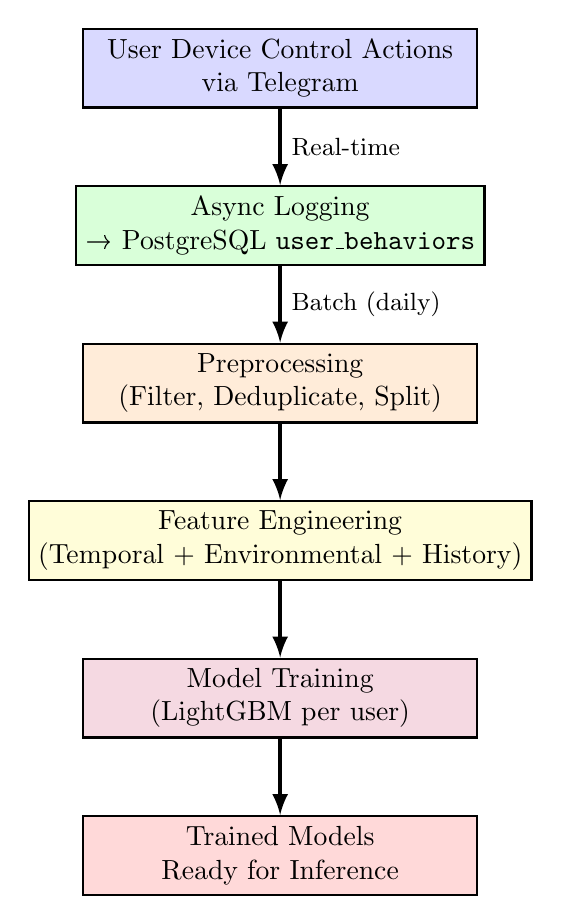
\begin{tikzpicture}[
        node distance=1.8cm,
        box/.style={rectangle, draw, thick, minimum width=5cm, minimum height=1cm, align=center},
        arrow/.style={-latex, thick}
    ]
        % Vertical flow - clean and simple
        \node[box, fill=blue!15] (user) at (0, 0) {User Device Control Actions\\via Telegram};
        
        \node[box, fill=green!15] (log) at (0, -2) {Async Logging\\→ PostgreSQL \texttt{user\_behaviors}};
        
        \node[box, fill=orange!15] (preprocess) at (0, -4) {Preprocessing\\(Filter, Deduplicate, Split)};
        
        \node[box, fill=yellow!15] (features) at (0, -6) {Feature Engineering\\(Temporal + Environmental + History)};
        
        \node[box, fill=purple!15] (train) at (0, -8) {Model Training\\(LightGBM per user)};
        
        \node[box, fill=red!15] (deploy) at (0, -10) {Trained Models\\Ready for Inference};
        
        % Arrows
        \draw[arrow, ultra thick] (user) -- node[right, font=\small] {Real-time} (log);
        \draw[arrow, ultra thick] (log) -- node[right, font=\small] {Batch (daily)} (preprocess);
        \draw[arrow, ultra thick] (preprocess) -- (features);
        \draw[arrow, ultra thick] (features) -- (train);
        \draw[arrow, ultra thick] (train) -- (deploy);
        
    \end{tikzpicture}
    \caption{Data pipeline for behavior learning. User actions are logged in real-time, then processed in nightly batch jobs to train per-user models.}
    \label{fig:data-pipeline-clean}
\end{figure}

\subsection{Training Protocol and Evaluation Metrics}
\label{sec:training-eval}

\subsubsection{Training configuration}

Each user's model is trained independently using the following configuration:

\begin{itemize}
    \item \textbf{Algorithm:} LightGBM with gradient-based one-side sampling (GOSS)
    \item \textbf{Objective:} Multi-class cross-entropy for device prediction; MSE for state regression
    \item \textbf{Number of trees:} 100 (early stopping if validation loss does not improve for 20 rounds)
    \item \textbf{Learning rate:} 0.1
    \item \textbf{Max tree depth:} 6
    \item \textbf{Regularization:} L2 leaf regularization ($\lambda = 1.0$)
    \item \textbf{Min data in leaf:} 20 (prevents overfitting on small datasets)
\end{itemize}

Training completes in 2--10 seconds per user on a CPU (Intel i7, 16GB RAM), making nightly retraining computationally feasible.

\subsubsection{Evaluation metrics}

Model performance is assessed using multiple complementary metrics:

\paragraph{Device prediction (classification)}
\begin{itemize}
    \item \textbf{Top-1 Accuracy:} Fraction of times the predicted device matches the user's actual next action. Target: $>$50\% (chance baseline: 1/M where M = number of devices).
    
    \item \textbf{Top-3 Accuracy:} Fraction of times actual device is in top 3 predictions. Target: $>$80\%.
    
    \item \textbf{Macro-averaged F1:} Harmonic mean of precision and recall across all device classes. Accounts for class imbalance (some devices used more frequently than others).
\end{itemize}

\paragraph{State prediction (regression)}
\begin{itemize}
    \item \textbf{Mean Absolute Error (MAE):} For continuous controls (brightness), measures average deviation from user's preferred value. Target: $<$10\% (e.g., if user prefers 70\%, prediction within [63, 77] is acceptable).
    
    \item \textbf{R² Score:} Explains fraction of variance in preferred states captured by the model. Target: $>$0.6.
\end{itemize}

\paragraph{Business metrics}
\begin{itemize}
    \item \textbf{Suggestion acceptance rate:} Fraction of proactive suggestions (``Turn on light?'') that user accepts within 5 minutes. Target: $>$30\%.
    
    \item \textbf{False positive rate:} Fraction of suggestions rejected or ignored. Must be $<$20\% to avoid user annoyance.
\end{itemize}

\subsubsection{Baseline comparisons}

To validate the model's effectiveness, performance is compared against three baselines:

\begin{enumerate}
    \item \textbf{Random baseline:} Uniform random selection from available devices. Establishes lower bound.
    
    \item \textbf{Frequency baseline:} Always predict the device most frequently used by the user, regardless of context. Tests whether contextual features add value.
    
    \item \textbf{Time-based baseline:} Predict device based only on time-of-day statistics (``At 6:30 AM, user typically controls living room light''). Tests whether environmental context improves beyond temporal patterns alone.
\end{enumerate}

Ablation studies quantify the contribution of each feature group (temporal, environmental, historical) by training models with progressively more feature sets and measuring performance gains.

\subsection{Continuous Learning Mechanism}
\label{sec:continuous-learning}

User preferences evolve over time due to seasonal changes, lifestyle shifts, or acquisition of new devices. The system implements a continuous learning pipeline to adapt models without manual intervention.

\subsubsection{Nightly retraining schedule}

At 3:00 AM daily, an automated batch job:

\begin{enumerate}
    \item Extracts all new behavior logs from the past 24 hours
    \item Appends new data to each user's training set
    \item Retrains models using updated datasets
    \item Evaluates on holdout test set (most recent 15\% of data)
    \item If test performance degrades by $>$10\% compared to previous version, triggers alert for manual investigation (potential data quality issue or distribution shift)
    \item Exports trained models to disk (\texttt{/models/user\_\{id\}\_v\{timestamp\}.lgb})
    \item Hot-reloads new models into the PersonalizationAgent without restarting the backend service
\end{enumerate}

\subsubsection{Concept drift detection}

To detect when user behavior fundamentally changes (concept drift), the system monitors two indicators:

\begin{itemize}
    \item \textbf{Validation loss trend:} If loss increases monotonically for 7 consecutive days, indicates model is no longer capturing current patterns.
    
    \item \textbf{Feature distribution shift:} KL-divergence between feature distributions in training window (30 days) vs recent window (7 days). Threshold: $D_{KL} > 0.5$ triggers retraining from scratch with only recent data.
\end{itemize}

\subsubsection{Cold start for new users}

When a new user joins the household, they have no historical data. The system handles cold start through:

\begin{enumerate}
    \item Use a \textbf{global default model} trained on all users' data (if available). This model captures general household patterns but lacks personalization.
    
    \item After collecting 50+ actions ($\sim$5--10 days of typical usage), train an initial personal model.
    
    \item Gradually transition from global to personal model: blend predictions $\hat{y} = \alpha \cdot \hat{y}_{\text{global}} + (1 - \alpha) \cdot \hat{y}_{\text{personal}}$ where $\alpha$ decays from 1 to 0 as personal dataset grows.
\end{enumerate}

This three-phase approach (global → blended → personal) balances cold-start performance with rapid personalization as data accumulates.

%%%%%%%%%%%%%%%%%%%%%%%%%%%%%%%%%%%%%%%%%%%%%%%%%%%%%%%%%%%%%%%%%%%%%%%
% PART B: SYSTEM ENGINEERING
%%%%%%%%%%%%%%%%%%%%%%%%%%%%%%%%%%%%%%%%%%%%%%%%%%%%%%%%%%%%%%%%%%%%%%%

\subsection*{\Large PART B: SYSTEM ENGINEERING}
\addcontentsline{toc}{subsection}{Part B: System Engineering}

\subsection{Multi-User Context Management}
\label{sec:multiuser-context}

A key engineering challenge is handling multiple users issuing concurrent requests to a single HERA LLM backend. This section describes how per-user personalization is achieved without requiring separate agent instances.

\subsubsection{UserContext data structure}

When a message arrives from Telegram, the orchestrator constructs a \texttt{UserContext} object containing:

\begin{verbatim}
class UserContext:
    user_id: int              # Database primary key
    chat_id: str              # Telegram chat ID
    name: str                 # Display name (e.g., "Dad")
    role: str                 # "admin", "member", or "guest"
    recent_actions: List[Action]  # Last 10 actions
    learned_preferences: Dict[str, Any]  # Cached patterns
    active_since: datetime    # When user last interacted
\end{verbatim}

This context is loaded once per request (latency $\sim$5ms for database lookup) and passed to all specialist agents.

\subsubsection{Context injection mechanism}

The orchestrator injects UserContext into agent system prompts using a template:

\begin{verbatim}
System Prompt Template:
---
You are assisting {user.name} (role: {user.role}).
Their typical preferences:
- Preferred brightness: {user.preferences.brightness}
- Usually active between {user.preferences.active_hours}
- Recent pattern: {user.recent_actions}

Current environment:
- Temperature: {env.temperature}°C
- Devices: {env.device_states}
---
\end{verbatim}

This allows the LLM to generate personalized responses (``I've set the light to 70\%, your usual preference'') without maintaining per-user agent instances.

Figure~\ref{fig:multiuser-handling} illustrates the request flow for multi-user scenarios.

\begin{figure}[H]
    \centering
    \begin{tikzpicture}[
        node distance=1.5cm,
        box/.style={rectangle, draw, thick, minimum width=5cm, minimum height=0.9cm, align=center},
        arrow/.style={-latex, thick}
    ]
        % Vertical flow - single HERA instance handling multiple users
        \node[box, fill=blue!15] (users) at (0, 0) {User 1, User 2, User 3\\(concurrent Telegram messages)};
        
        \node[box, fill=purple!15] (telegram) at (0, -1.8) {Telegram Adapter\\Receives \texttt{chat\_id}};
        
        \node[box, fill=orange!15] (orchestrator) at (0, -3.6) {Orchestrator\\Loads UserContext for chat\_id};
        
        \node[box, fill=yellow!15] (pers_agent) at (0, -5.4) {PersonalizationAgent\\Loads User's ML Model (lazy)};
        
        \node[box, fill=green!15] (inference) at (0, -7.2) {Model Inference\\Predicts next action + state};
        
        \node[box, fill=red!15] (response) at (0, -9) {Personalized Response\\``Set light to 70\%, your usual''};
        
        % Arrows
        \draw[arrow, ultra thick] (users) -- (telegram);
        \draw[arrow, ultra thick] (telegram) -- (orchestrator);
        \draw[arrow, ultra thick] (orchestrator) -- (pers_agent);
        \draw[arrow, ultra thick] (pers_agent) -- (inference);
        \draw[arrow, ultra thick] (inference) -- (response);
        
        % Side note
        \node[right=0.5cm of orchestrator, text width=4cm, font=\footnotesize, align=left] {
            \textbf{Single LLM instance}\\
            Context switched\\
            per request
        };
        
    \end{tikzpicture}
    \caption{Multi-user handling with single HERA instance. UserContext is loaded per request and injected into agent prompts, enabling personalization without separate instances.}
    \label{fig:multiuser-handling}
\end{figure}

\subsubsection{Model caching strategy}

Loading a LightGBM model from disk takes $\sim$20ms, which is acceptable for first request but undesirable for subsequent requests. The system implements an LRU (Least Recently Used) cache:

\begin{itemize}
    \item Cache capacity: 5 models (suitable for family households with 3--5 members)
    \item Cache key: \texttt{user\_id}
    \item Eviction policy: When cache is full, evict least recently used model
    \item Cache hit rate: Typically $>$95\% in family scenarios (users issue requests in bursts)
\end{itemize}

This reduces average model loading time from 20ms to $<$1ms (in-memory lookup).

\subsection{Integration with HERA Architecture}
\label{sec:hera-integration}

The PersonalizationAgent is implemented as a specialist agent within the existing HERA orchestrator-specialist topology (described in Section~\ref{sec:multi-agent}).

\subsubsection{Agent responsibilities}

The PersonalizationAgent handles three types of requests:

\begin{enumerate}
    \item \textbf{Reactive personalization:} When DeviceAgent receives ambiguous commands (``turn on light'' without brightness), it queries PersonalizationAgent for user's preferred state.
    
    \item \textbf{Proactive suggestions:} Background inference runs every 10 minutes. If prediction confidence exceeds threshold ($P(\text{device}) > 0.75$) and user has not recently received a suggestion, generate proactive message.
    
    \item \textbf{Explanation queries:} User can ask ``Why did you suggest that?'' and PersonalizationAgent provides SHAP-based explanations (``You typically turn on the bedroom light around this time on weekdays'').
\end{enumerate}

\subsubsection{Conflict resolution}

When multiple users issue conflicting commands within a short time window (30 seconds), the system applies a resolution hierarchy:

\begin{enumerate}
    \item \textbf{Role-based priority:} Admin $>$ Member $>$ Guest. If users have different roles, higher role wins.
    
    \item \textbf{Temporal priority:} Most recent command takes precedence (last-write-wins policy).
    
    \item \textbf{Negotiated compromise:} For continuous controls (brightness, temperature), compute weighted average: $s_{\text{final}} = w_1 \cdot s_1 + w_2 \cdot s_2$ where weights are proportional to user roles.
    
    \item \textbf{LLM-mediated resolution:} If automatic resolution is ambiguous, orchestrator asks LLM to generate a mediation message: ``Dad wants light at 100\%, Mom wants it off. Setting to 50\% as compromise. Override?''
\end{enumerate}

This hierarchy ensures fair multi-user coexistence while respecting household authority structures.

\subsection{Summary}

This chapter presented a complete machine learning system for learning and predicting user behavior in a multi-user smart home environment. The key contributions are:

\begin{enumerate}
    \item \textbf{Model selection and justification:} LightGBM is chosen for its data efficiency, fast inference, and interpretability. Empirical comparisons and ablation studies validate this choice.
    
    \item \textbf{Feature engineering:} A compact 20-dimensional feature set captures temporal patterns, environmental context, and user history, balancing expressiveness with overfitting risk.
    
    \item \textbf{Continuous learning:} Automated nightly retraining and concept drift detection enable models to adapt to evolving user preferences without manual intervention.
    
    \item \textbf{Multi-user engineering:} Single LLM instance handles multiple users through UserContext injection and lazy model loading, achieving personalization without architectural fragmentation.
\end{enumerate}

The system transforms the smart home from a passive command executor into an adaptive assistant that learns each household member's preferences and proactively supports their daily routines.
